\documentclass[12pt, letterpaper]{article}
\usepackage{graphicx} % Required for inserting images
\usepackage[utf8]{inputenc}
\usepackage[margin=1in]{geometry}
\usepackage{booktabs}
\usepackage{tabu}
\usepackage[labelfont=bf, skip=5pt, font=small]{caption}
\usepackage{subcaption}
\usepackage{fancyhdr}
\usepackage{amsmath}

\setlength{\parskip}{1em}
\setlength{\parindent}{0em}

\begin{document} 
\begin{center}
    \huge{Ohm's Law Lab Report} \\[10pt]
    \large{Jamhad D. Byers}
\end{center}
\rule{\textwidth}{0.5pt}
\begin{abstract}
    \noindent A statement within Ohm’s Law is that the current through a resistor is proportional to the voltage across the resistor. Using a current probe to measure the current through a wire and a voltage probe to measure potential difference across a resistor, we can test the validity of this statement. If such a statement were true, the graphic behavior of voltage and current should show strong proportionality. Indeed, it is the case for resistors in a circuit, but not for a light bulb.
\end{abstract}
\rule{\textwidth}{0.5pt}

\section{Introduction \& Background}

The purpose of this experiment was to evaluate the mathematical relationship between current, potential difference, and resistance in a simple circuit while also comparing the potential vs. current behavior for a resistor and a light bulb. Because Ohm's Law assumes constant temperature, the resistors are presumed to behave according to this law, but the bulb should not, given the fact that the increase in temperature is what causes the bulb to light to begin with.

\section{Methods}

\begin{table}[h]
    \centering
    \caption{Resistors \& summery of data collected}
    \begin{tabu}{*{4}{X[c]}}
        \toprule
         \textbf{Resistor Listed Rating} & \textbf{Resistor Measured Rating} & \textbf{Slope of Regression Line (V/A)} & \textbf{Y-intercept of Regression Line (V)} \\
        \midrule
         100 Ohms & 101.0 Ohms & 99.28 V/A & 0.01 V \\
         200 Ohms & 198.6 Ohms & 199.10 V/A & 0.01 V \\
         \bottomrule
    \end{tabu}
    \label{tab:Data Table}
\end{table}

Resistors have resistance ratings given by their manufacturers, but the actual value is within a certain tolerance, here it is assumed to be 10\%. This means each resistor has an actual value falls within a 10\% increase or decrease range. Indeed, they measured values do fall within this range. After measuring the resistance of each resistor to be tested, a voltage is run through the circuit containing the resistor. This voltage starts at 0.5 volts and is increased by 0.5 volts until the maximum testing voltage for this experiment is reached, that being 5.0 volts. For each increment of voltage increase, the corresponding increase in current is mapped on a current vs. voltage graph for each resistor. A brief summery of the data collected from each resistor is listen in table \ref{tab:Data Table}. It is important to note the proportionality (slope) constant of each resistor is very close to their measured value and also falls within the tolerance range of each. This is because that constant is a measure of the resistance of each resistor. The percent difference can be calculated as follows:

\begin{equation}
    \% Difference = \frac{\lvert \Omega_m - \Omega_p \rvert}{\frac{1}{2}(\Omega_m + \Omega_p)} \cdot 100
\end{equation}

The resulting percent difference for the 100 ohm resistor is 1.72\% and for the 200 ohm resistor, 0.25\%. Once the data on the resistors was collected, a circuit containing a light bulb is constructed with the same current probe and voltage probe set-up. The steps are repeated as before, except now with an important distinction; the voltage is initially only increased in increments of 0.1 volts (up to the 1 volt mark) to truly capture a particular property of the circuit. Where there was a linear appearance to the normal resistor graphs tested, the light bulb’s potential vs. current graph is curved upward. Initially as the voltage increases, the current through the bulb shows minimal growth. After the voltage is increased beyond 1 volt, the linear proportionality of the two properties begins to emerge again.

\section{Results, Discussion \& Conclusion}

Below are the graphs corresponding to each resistor, as well as the light bulb and the graph displaying the change in resistance values with the increase in voltage through the light bulb.


\begin{figure}[h]
    \centering
    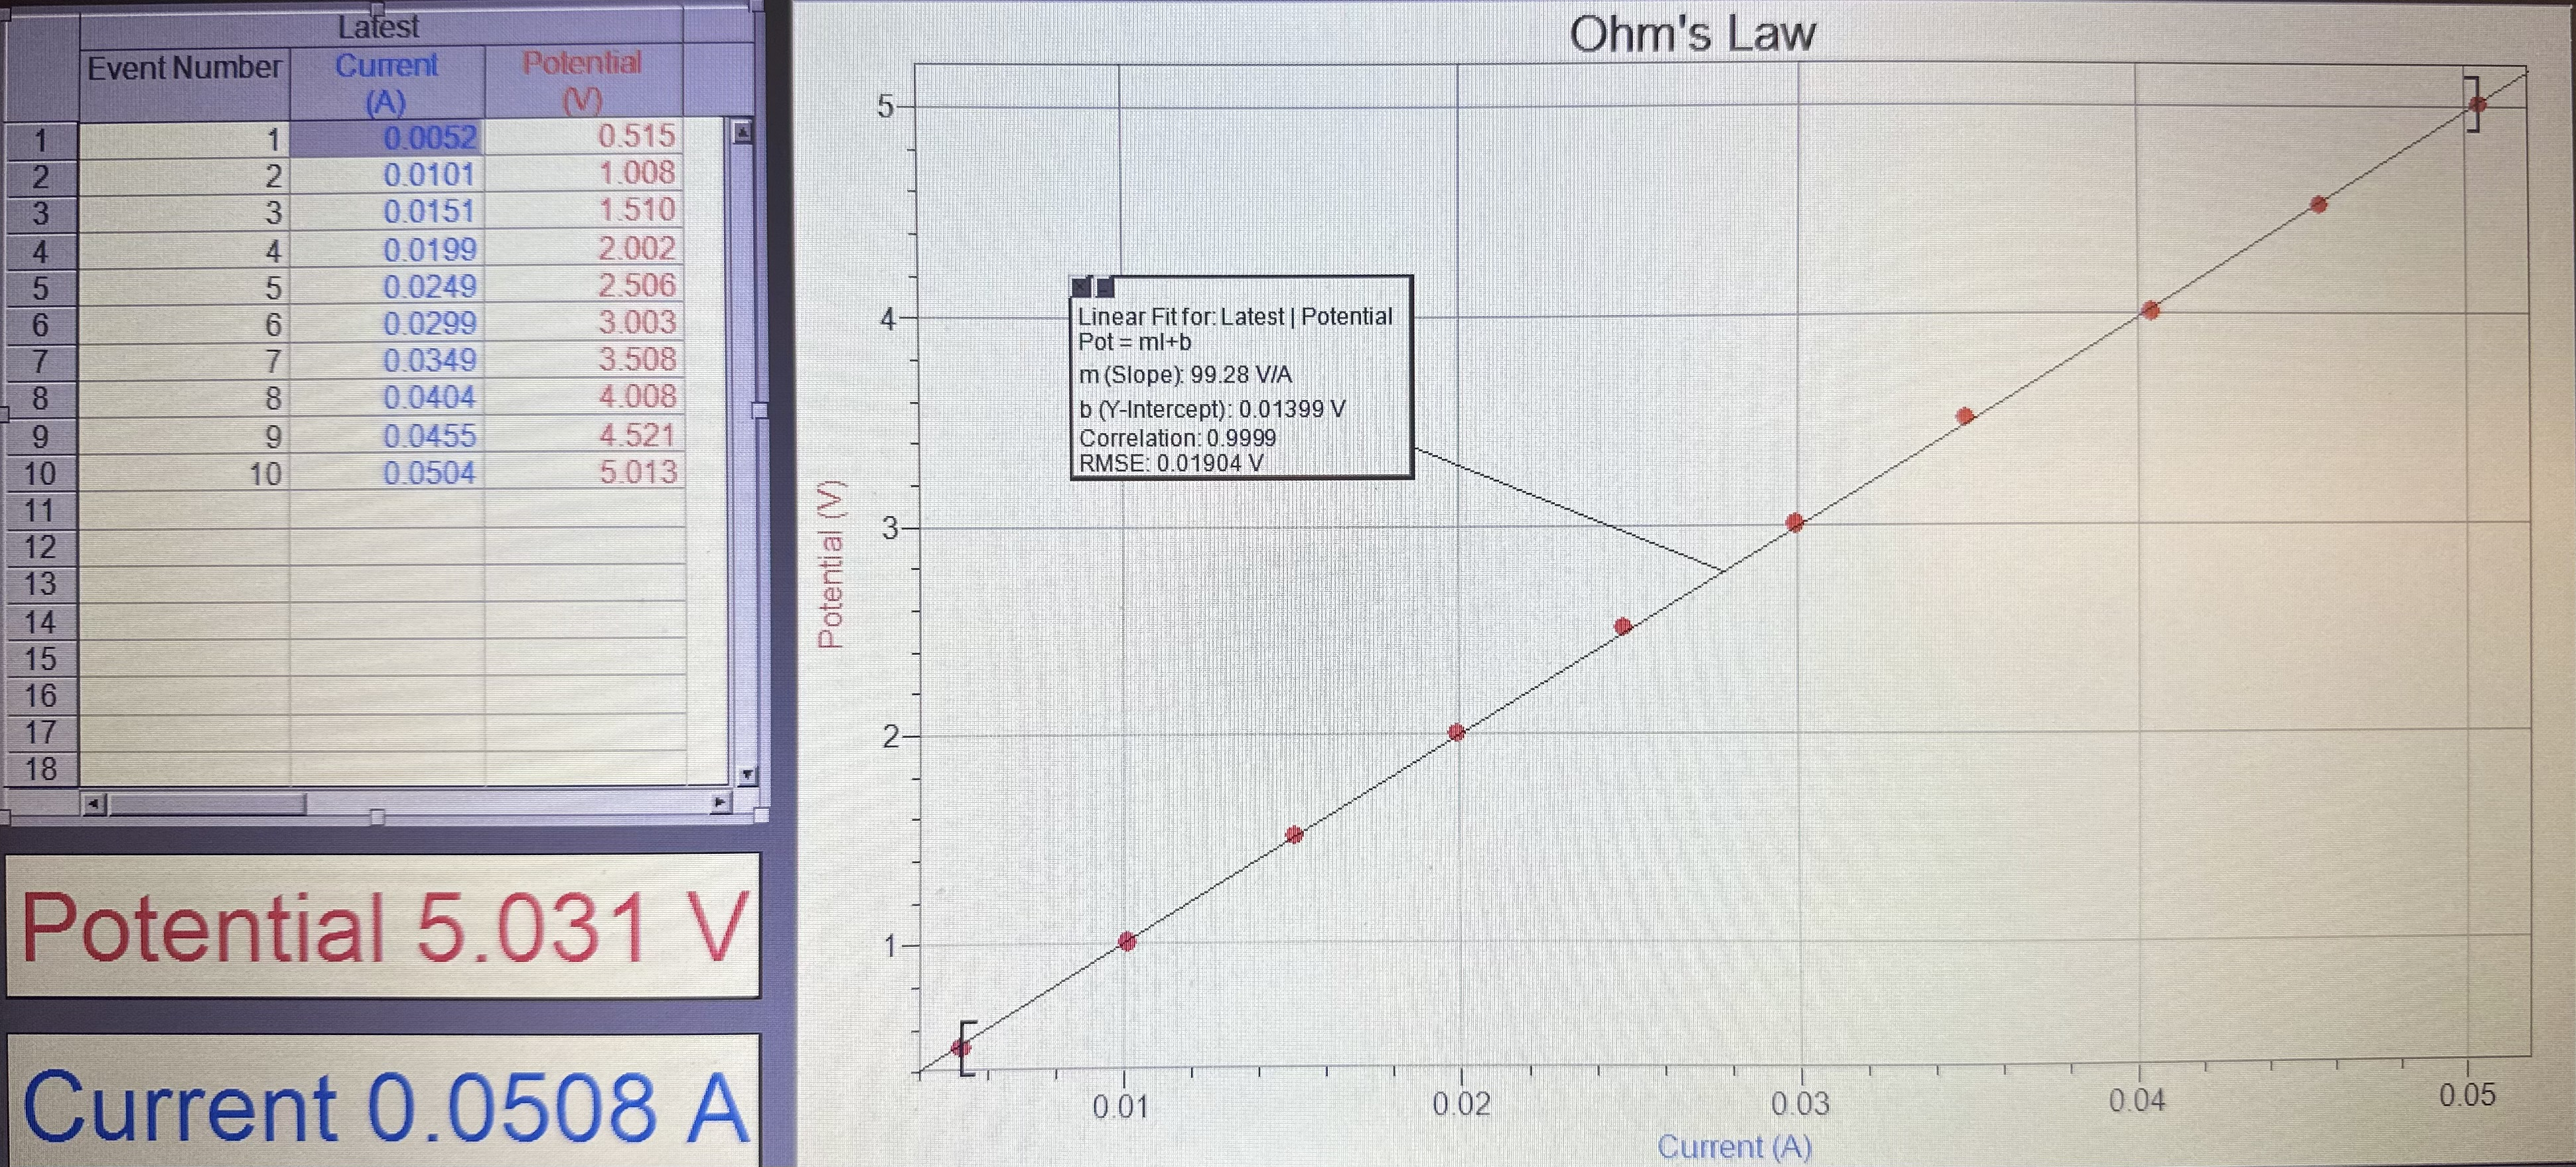
\includegraphics[width=\textwidth]{101.0_Resistor.JPG}
    \caption{100 Ohm resistor voltage vs current graph}
\end{figure}
\begin{figure}[h!]
    \centering
    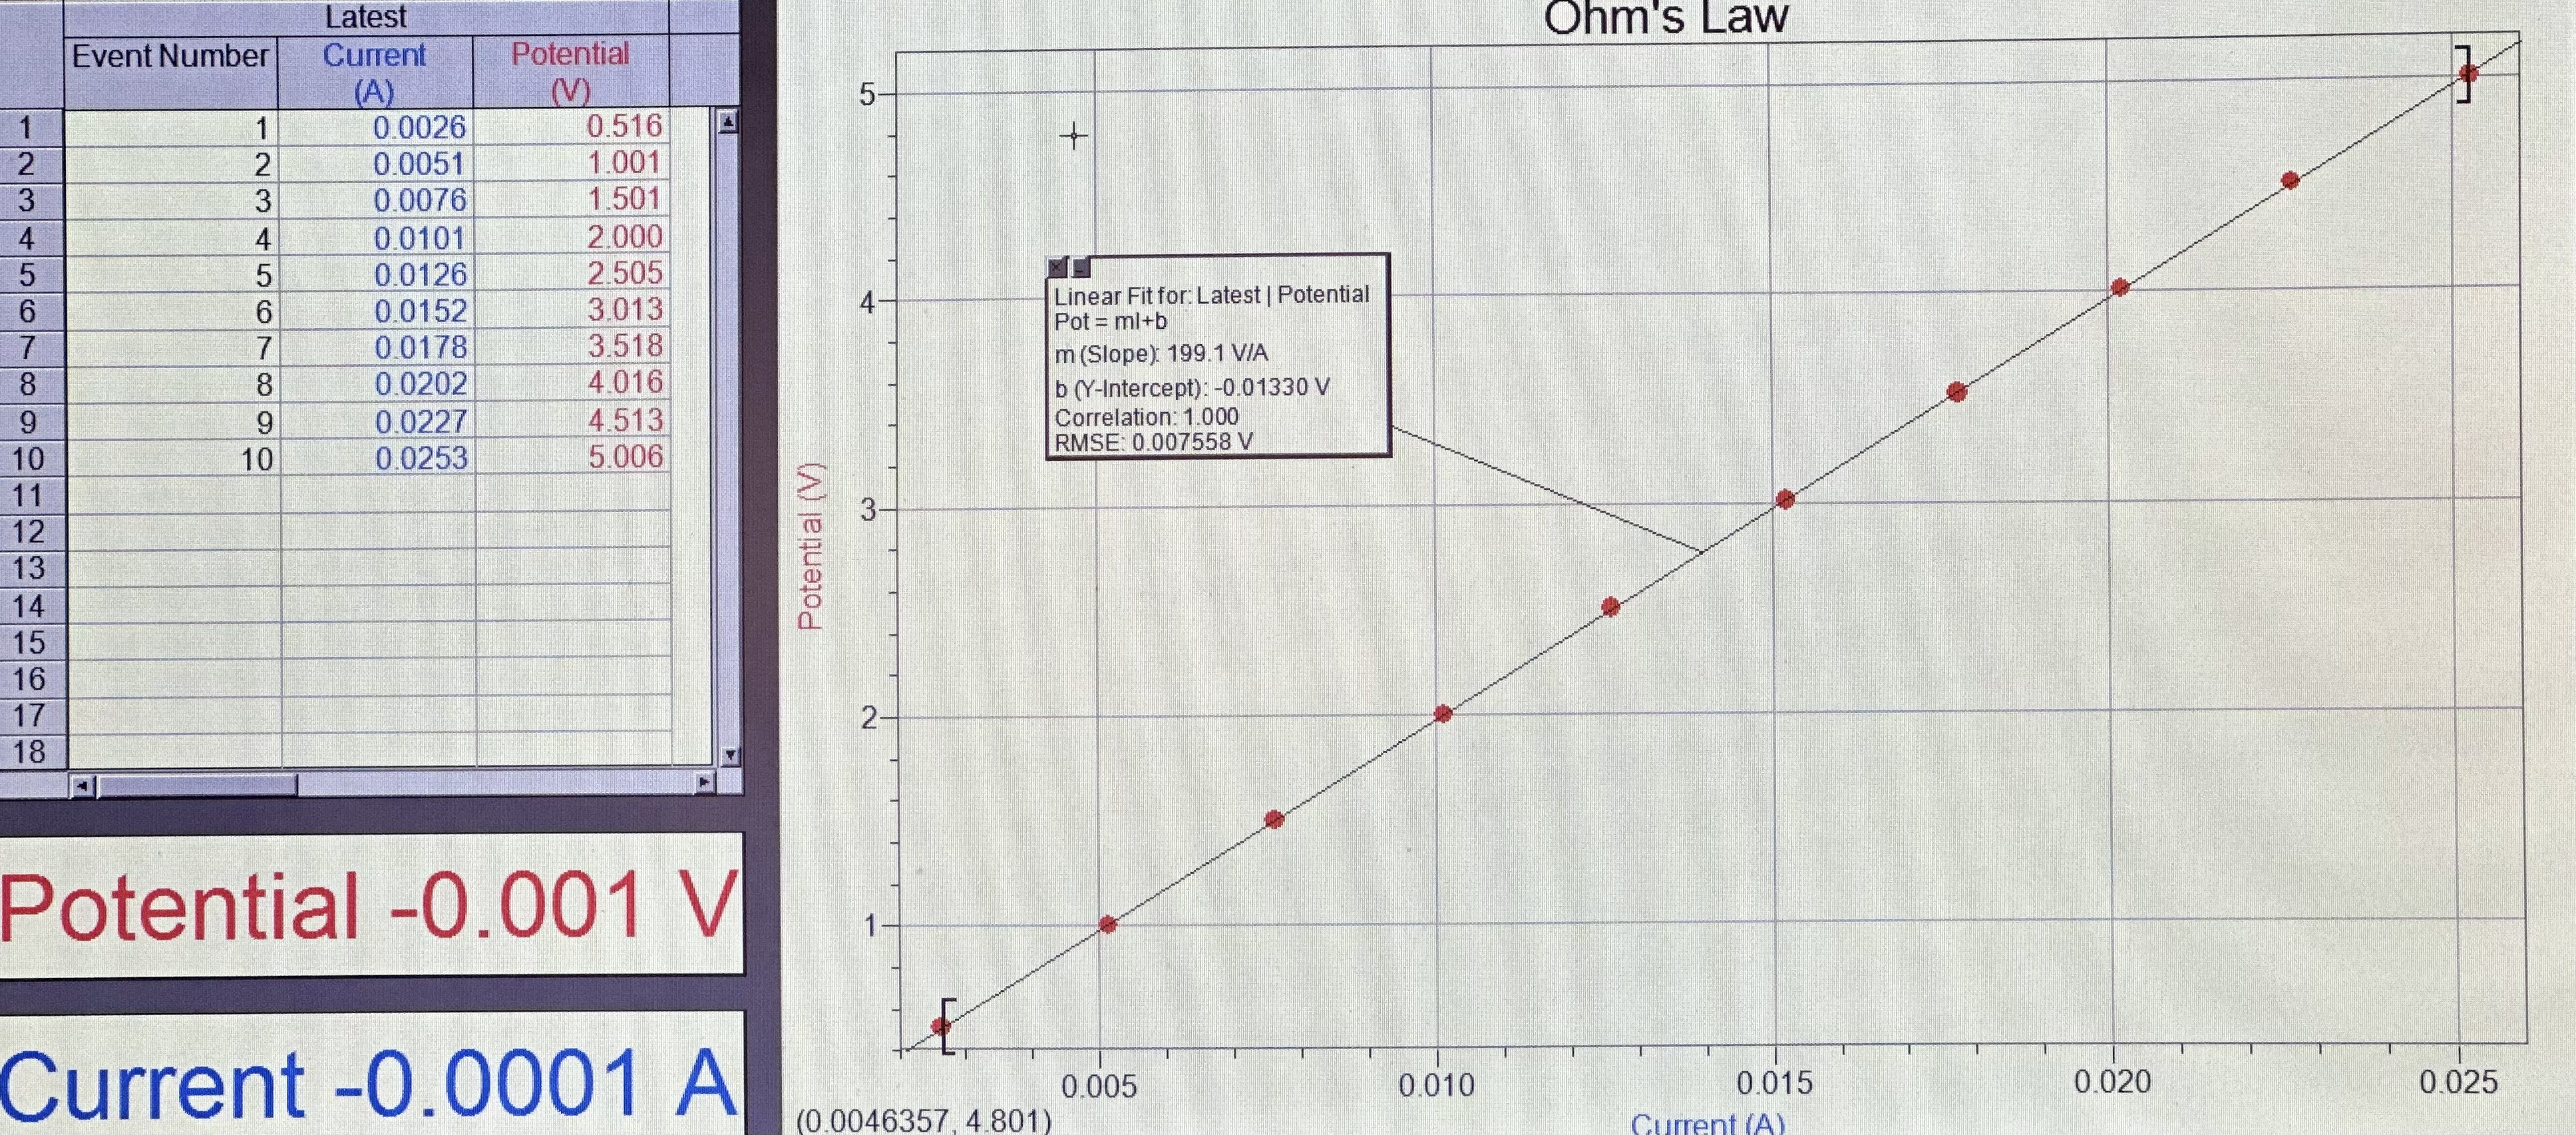
\includegraphics[width=\textwidth]{198.6_Resistor.JPG}
    \caption{200 Ohm resistor voltage vs current graph}
\end{figure}
\begin{figure}[t!]
    \centering
    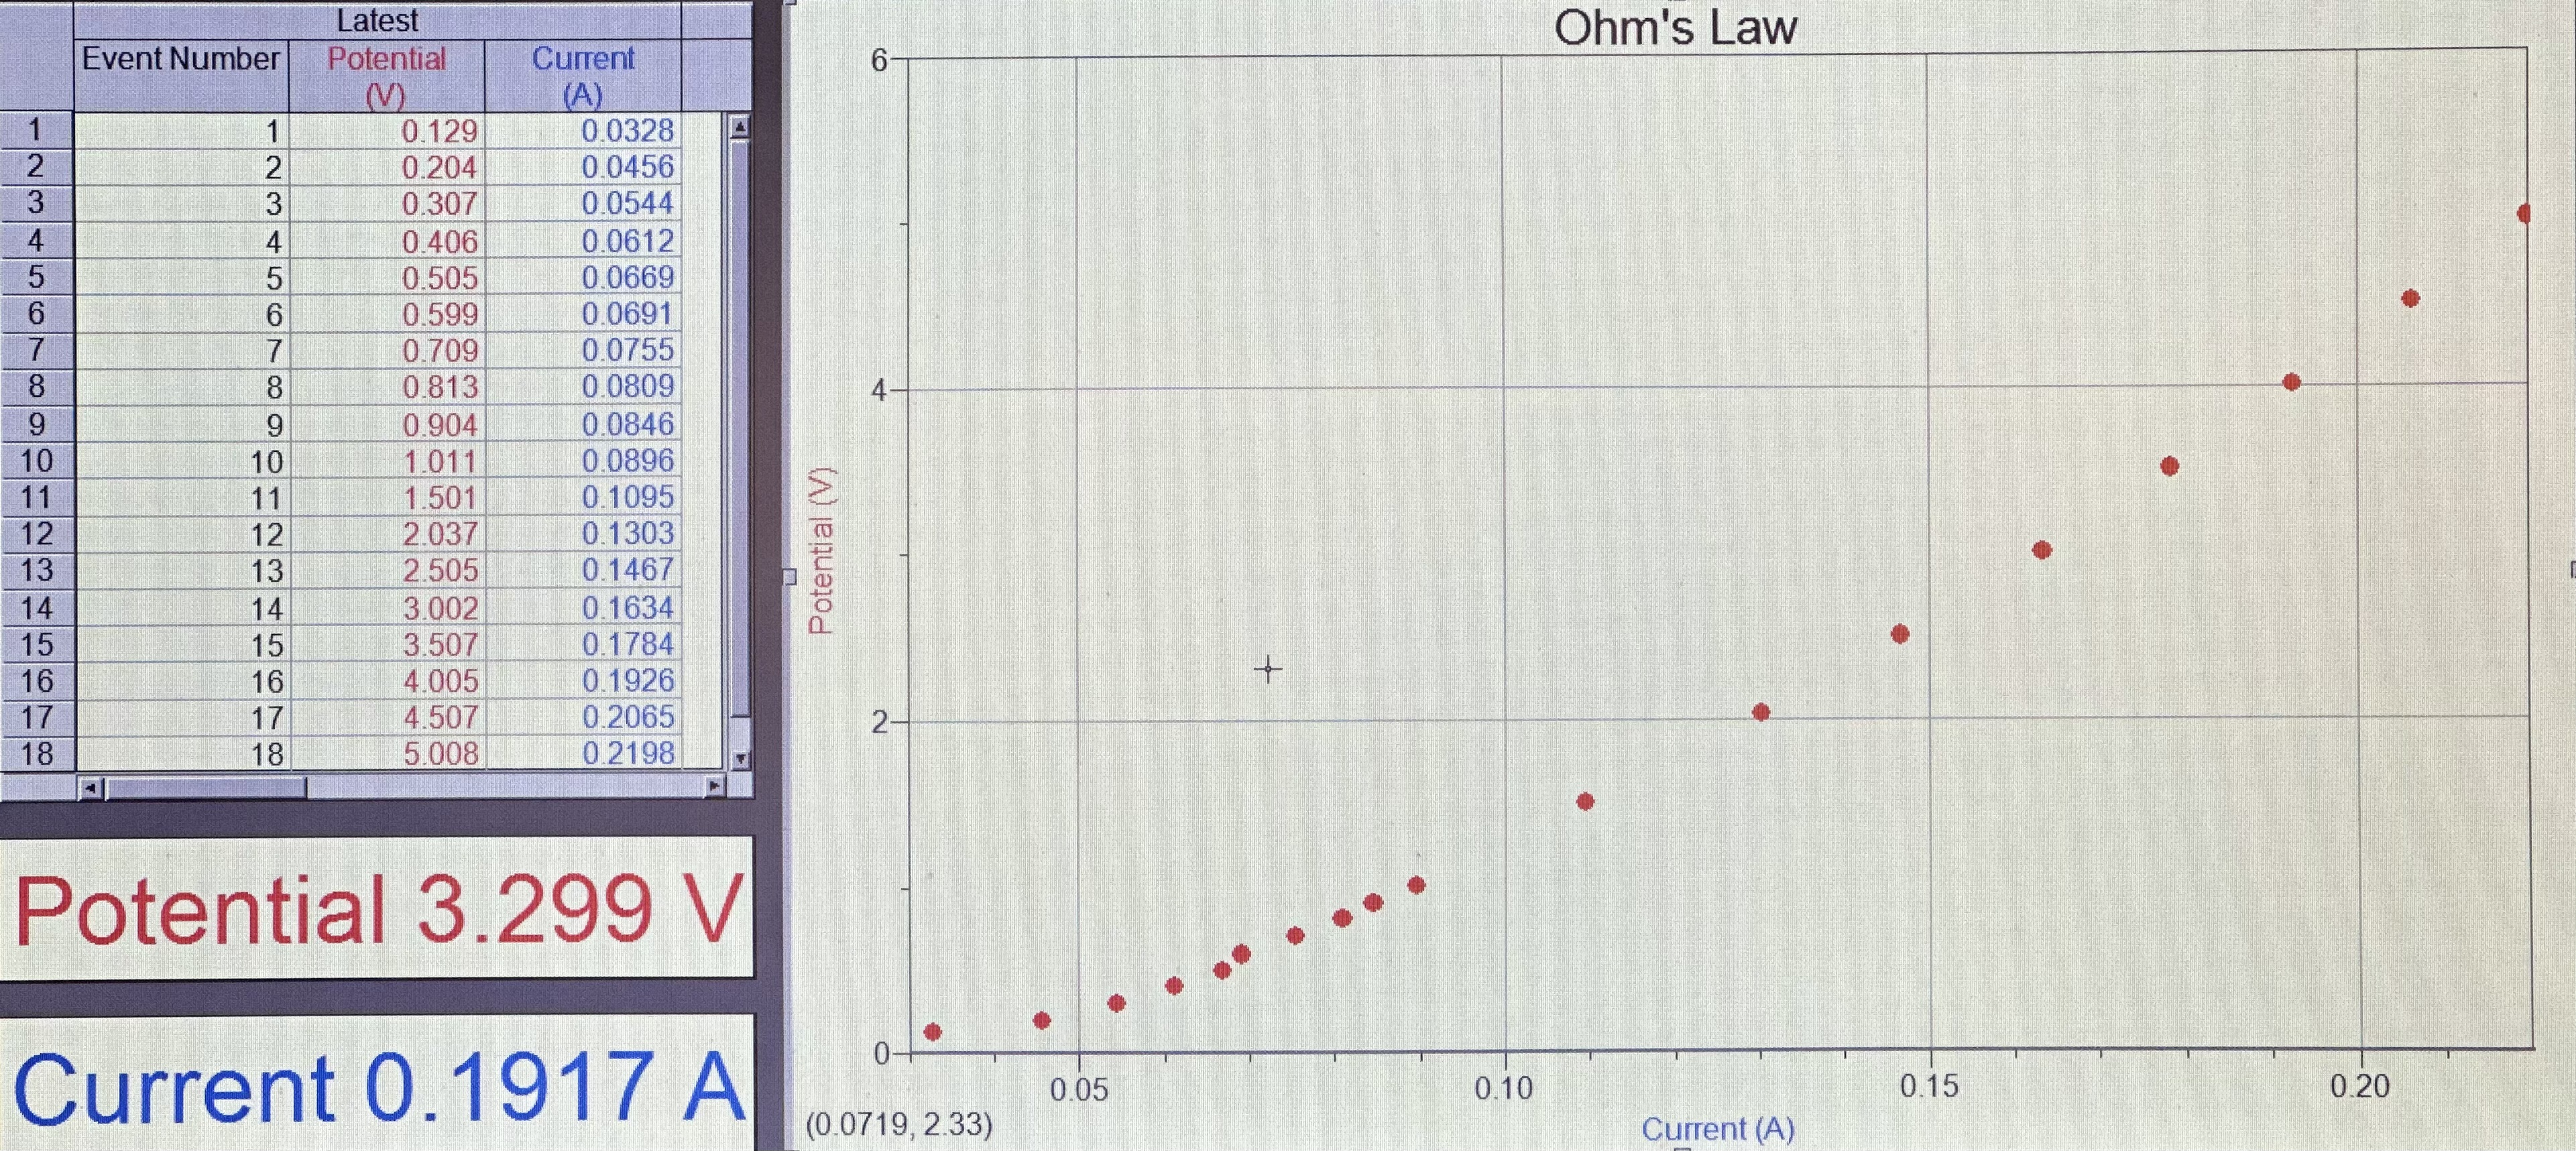
\includegraphics[width=\textwidth]{Light_Bulb.JPG}
    \caption{Light bulb voltage vs current graph}
\end{figure}
\begin{figure}[t!]
    \centering
    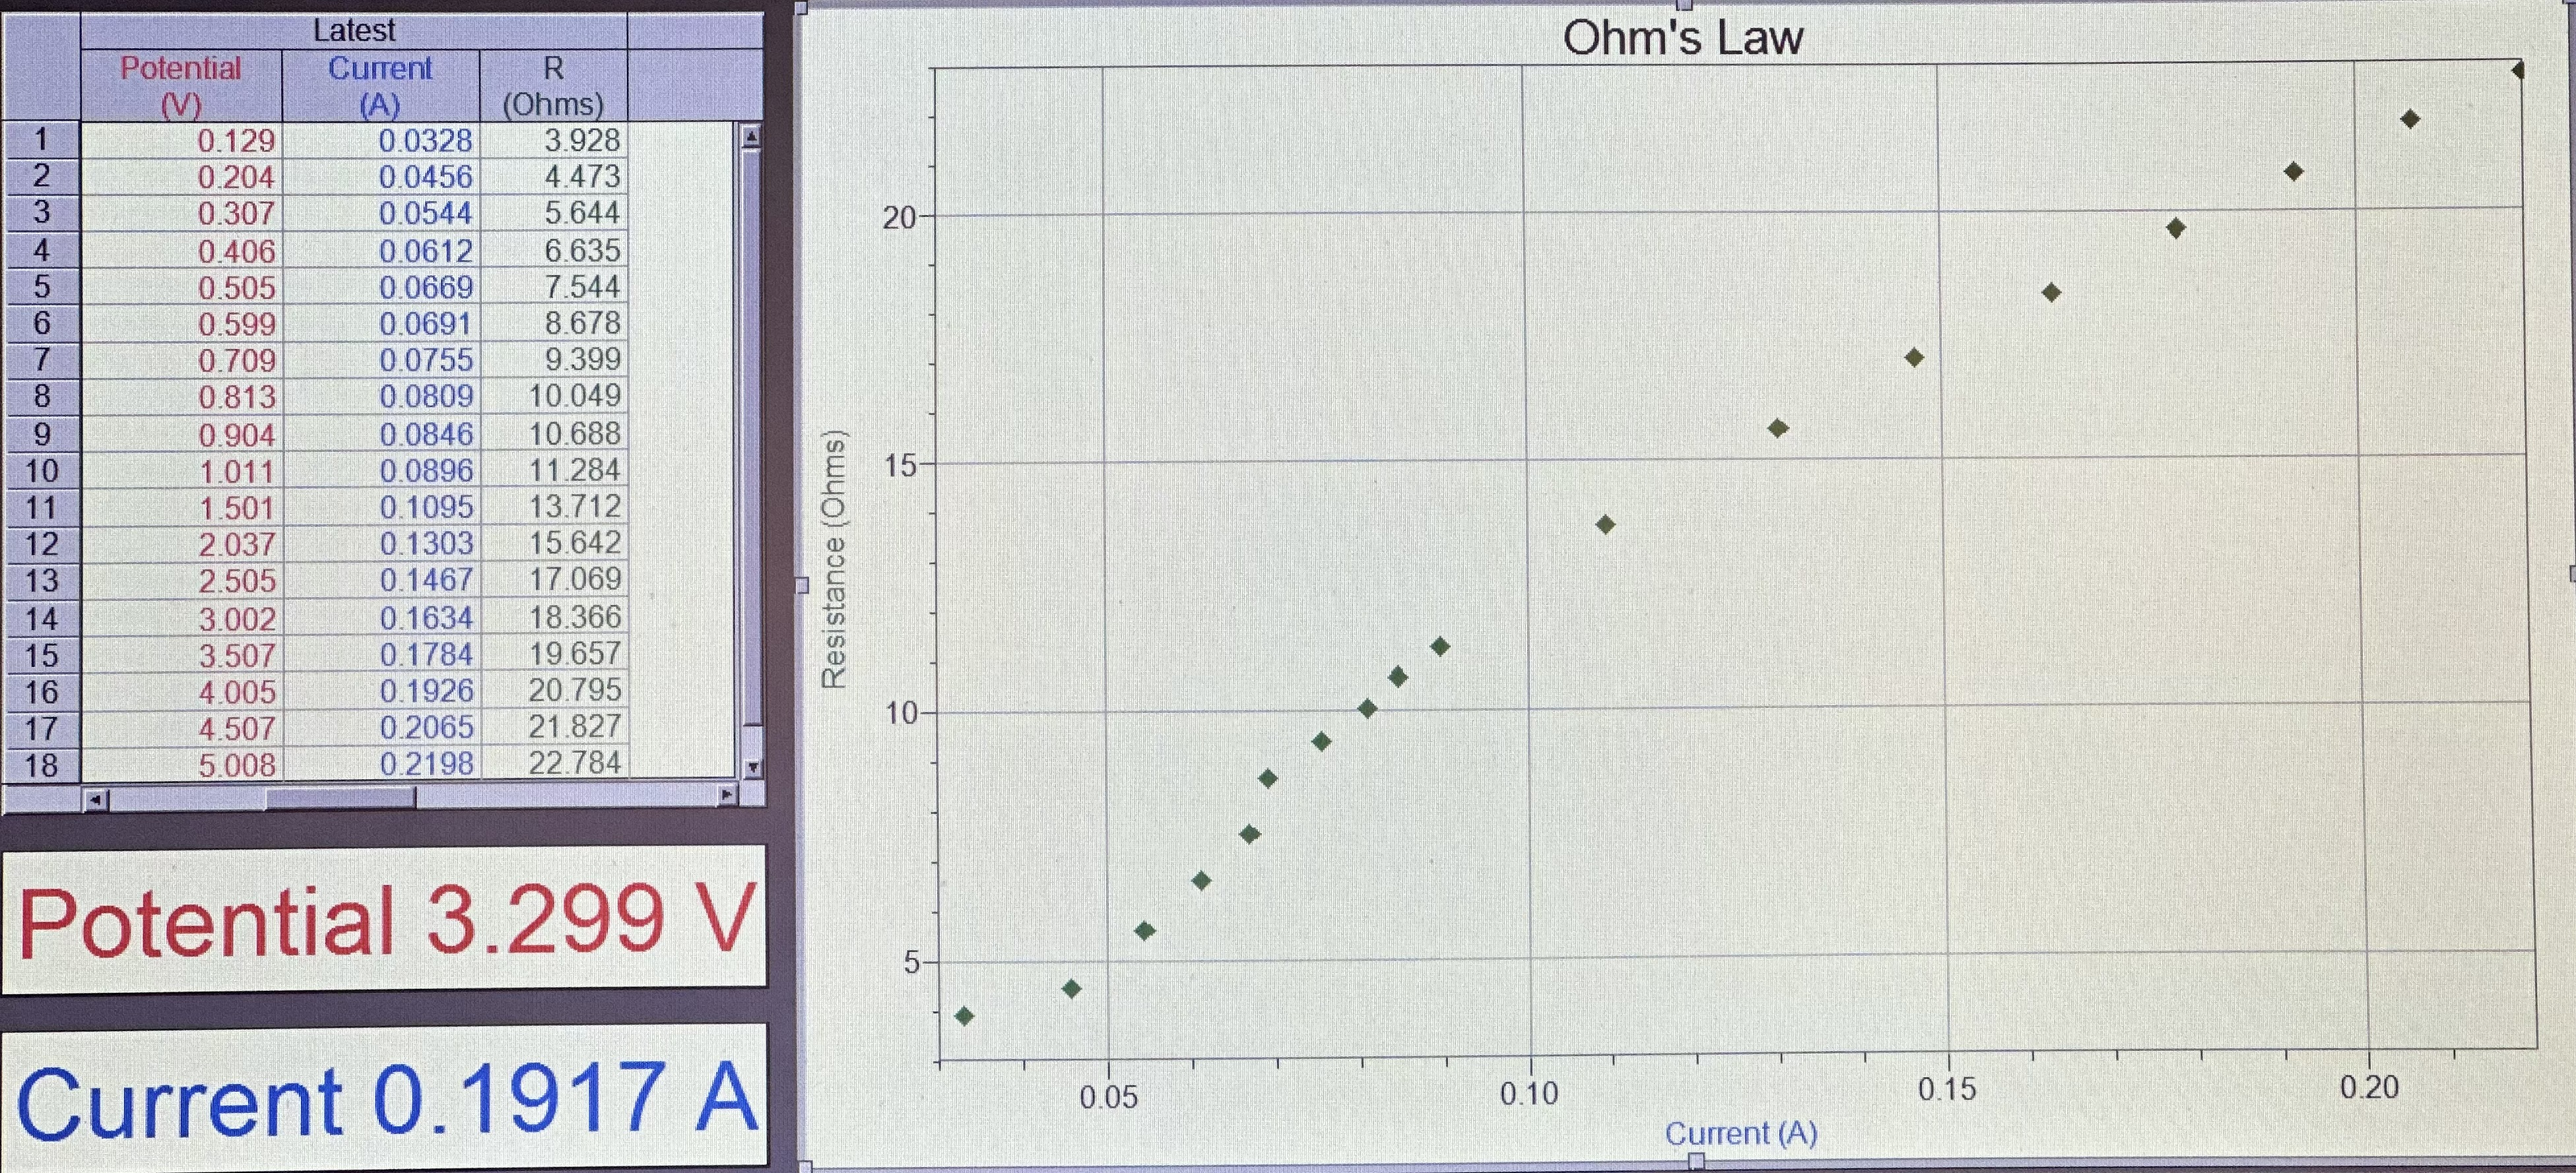
\includegraphics[width=\textwidth]{Resistance vs Current.JPG}
    \caption{Light bulb change in resistance graph}
\end{figure}

The resistors themselves behave as expected and have a constant proportionality, suggesting they are in fact ohmic devices. The non-linear appearance of the light bulb voltage vs current graph shows that it has a varying resistance as current increases, suggesting it is not an ohmic device because it does not follow Ohm's Law. Figure 4 gives a quantitative measure of how the resistance changes with increased current. It is also important to note why this happens. The current meets increased resistance as the bulb wire heats up because atoms are moving much more rapidly and the collision rate for how often electrons are impeded is increased and continues to increase with increased voltage. 

\end{document} 
